\documentclass[conference]{IEEEtran}
\IEEEoverridecommandlockouts
% The preceding line is only needed to identify funding in the first footnote. If that is unneeded, please comment it out.
\usepackage{cite}
\usepackage{amsmath,amssymb,amsfonts}
\usepackage{algorithmic}
\usepackage{graphicx}
\usepackage{textcomp}
\usepackage{xcolor}

\def\BibTeX{{\rm B\kern-.05em{\sc i\kern-.025em b}\kern-.08em
    T\kern-.1667em\lower.7ex\hbox{E}\kern-.125emX}}
\begin{document}



\title{Diabetes Prediction in the Pima Indian Female Population Evaluating Machine Learning Models\\}

\author{\IEEEauthorblockN{1\textsuperscript{st} Giorgio Saldana}
\IEEEauthorblockA{\textit{School of Science and Technology} \\
\textit{University of Camerino}\\
Camerino, Italy \\
giorgio.saldana@studenti.unicam.it}
\and
\IEEEauthorblockN{2\textsuperscript{nd} Marta Musso}
\IEEEauthorblockA{\textit{School of Science and Technology} \\
\textit{University of Camerino}\\
Camerino, Italy \\
marta.musso@studenti.unicam.it}
\and
\IEEEauthorblockN{3\textsuperscript{rd} Nabil Mohammed}
\IEEEauthorblockA{\textit{School of Science and Technology} \\
\textit{University of Camerino}\\
Camerino, Italy \\
nabilmohamme.khelifa@studenti.unicam.it}
\and
}

\maketitle

\begin{abstract}
This study investigates the application of machine learning techniques to predict diabetes mellitus in the Pima Indian population. Early diagnosis of diabetes, a significant global health concern, can lead to better management and outcomes. Using the Pima Indian Diabetes Female dataset from Kaggle, predictive models will be developed and evaluated to assist healthcare providers in making informed decisions. The high prevalence of diabetes in the Pima Indian population necessitates effective diagnostic tools. Traditional methods may not capture the complex factors of diabetes risk, whereas machine learning can analyze large datasets and identify subtle patterns for accurate and early prediction.

These models are expected to outperform conventional diagnostic methods in terms of accuracy and early detection capabilities. Specifically, integrating multiple health indicators, such as age, BMI, blood pressure, and glucose levels, into machine learning algorithms will result in higher predictive accuracy compared to single-factor analysis.
The study involves preprocessing data to handle missing values and outliers, selecting significant features, and developing predictive models using various machine learning algorithms. Model performance will be evaluated using accuracy, precision, recall, and AUC-ROC metrics, with cross-validation ensuring robustness and generalizability. 
We anticipate that our models will significantly enhance early detection and management of diabetes, ultimately improving patient outcomes.
\end{abstract}

\begin{IEEEkeywords}
Diabetes Prediction, Machine Learning, Pima Indian Female
\end{IEEEkeywords}

\section{Introduction}
Diabetes mellitus, commonly known as diabetes, is a group of metabolic disorders characterized by chronic high blood sugar levels due to insufficient insulin production or impaired insulin action. There are primarily three types of diabetes: Type 1, Type 2, and gestational diabetes. The complications of unmanaged diabetes are severe and include cardiovascular diseases, neuropathy, nephropathy, retinopathy, and increased risk of foot infections leading to amputations. Effective management typically involves lifestyle modifications, regular monitoring of blood glucose levels, and medications.

The Pima Indian population in Arizona exhibits one of the highest recorded rates of Type 2 diabetes globally, attributed to a combination of genetic predisposition and lifestyle factors. This unique dataset from the Pima Indian Diabetes dataset, available on Kaggle, includes health-related data such as age, BMI, blood pressure, and glucose levels, which are critical indicators of diabetes risk. The findings from this study will contribute to diabetes research and provide practical tools for healthcare professionals for early diagnosis and intervention strategies. By harnessing the power of machine learning (ML), this research aims to improve the quality of life for individuals at risk of diabetes and reduce the healthcare system's burden. This study aligns with the growing body of literature advocating for the integration of Artificial Intelligence (AI) and ML in medical diagnostics, promising more personalized and data-driven healthcare solutions \cite{Ref1}.

Recent advancements in ML and deep learning (DL) have shown significant potential in medical diagnostics, particularly for diseases like diabetes \cite{Ref2}. Various studies have demonstrated the effectiveness of models such as Logistic Regression (LR), Decision Trees (DT), Gradient Boosting Machines (GBM), and Support Vector Machines (SVM) in predicting diabetes \cite{Ref3}.

This research aims to explore the effectiveness of various ML models in predicting diabetes within the Pima Indian population. Specifically, it will investigate how factors like BMI, blood pressure, age, and glucose levels can be used to predict diabetes onset. By comparing the performance of different algorithms, including LR, DT, Random Forests (RF), SVM, and ensemble methods like GBM and XGBoost, this study seeks to identify the most accurate and reliable predictive models. The study will involve rigorous data preprocessing, feature selection, and model validation to ensure robust and reproducible results \cite{Ref4}.

It is expected that advanced ML models, such as RF and SVM, will outperform traditional statistical methods in predicting diabetes onset. Additionally, ensemble techniques like GBM and XGBoost are anticipated to enhance predictive accuracy by combining the strengths of multiple models \cite{Ref5}.

The remainder of this paper is structured as follows: Section II provides background information on diabetes mellitus and machine learning, establishing the foundation for our study. Section III describes the materials and methods used, including data preprocessing, feature selection, and the machine learning algorithms employed. Section IV details the development of the models, explaining the process and rationale behind each step. Section V presents the results, highlighting the performance metrics of the various models. Section VI reviews related works, comparing our approach and results with existing research in the field. Finally, Section VII concludes the study, summarizing the key contributions and suggesting directions for future research.

\section{Background}
\subsection{Diabetes Mellitus}
Diabetes mellitus is a chronic condition where the body cannot effectively regulate blood glucose levels due to insufficient insulin production or ineffective insulin action. There are three main types of diabetes:

\begin{itemize}
\item \textbf{Type 1 Diabetes:} An autoimmune condition where the immune system destroys insulin-producing beta cells in the pancreas, requiring lifelong insulin therapy. It is typically diagnosed in children and young adults.
\item \textbf{Type 2 Diabetes:} The most common form, associated with obesity and insulin resistance, primarily seen in adults. It involves either insufficient insulin production or cells being resistant to insulin.
\item \textbf{Gestational Diabetes:} Occurs during pregnancy when the body cannot produce enough insulin to meet increased needs. It usually resolves after childbirth but increases the risk of developing Type 2 diabetes later in life.
\end{itemize}

Managing diabetes involves regular monitoring of blood glucose levels, medication adherence, and lifestyle changes.

The Pima Indian population, particularly females, has one of the highest prevalence rates of Type 2 diabetes globally, attributed to genetic predisposition and lifestyle factors. Understanding these factors highlights the need for targeted research and intervention strategies to develop effective diagnostic tools and prevention programs.

%Diabetes mellitus is a chronic metabolic disorder characterized by elevated blood glucose levels due to insufficient insulin production, ineffective insulin action, or both. Insulin, a hormone produced by the pancreas, is crucial for regulating blood sugar levels. When insulin production is inadequate or the body cannot effectively use the insulin produced, glucose accumulates in the bloodstream, leading to hyperglycemia.
%Clinically, diabetes is classified into three main types: Type 1 diabetes, Type 2 diabetes, and gestational diabetes. 
%\begin{itemize}
    %\item Type 1 diabetes, this form is an autoimmune condition where the body's immune system attacks and destroys the insulin-producing beta cells in the pancreas. It is typically diagnosed in children and young adults. Patients with Type 1 diabetes require lifelong insulin therapy for glucose regulation.
    %\item Type 2 diabetes, this is the most common form, often associated with obesity and insulin resistance. In Type 2 diabetes, the body either does not produce enough insulin or the cells are resistant to insulin's effects. It is primarily seen in adults, but increasing rates are being observed in younger populations due to rising obesity rates.
    %\item Gestational diabetes, this type occurs during pregnancy when the body cannot produce enough insulin to meet the increased needs. Although it usually resolves after childbirth, it raises the risk of developing Type 2 diabetes later in life for both the mother and the child.
%\end{itemize}  
%The impact of diabetes on quality of life is profound. Managing diabetes requires constant monitoring of blood glucose levels, adherence to medication regimens, and lifestyle modifications. The burden of daily management, combined with the fear of complications, can lead to significant psychological stress, including anxiety and depression. Moreover, diabetes-related complications can result in physical disabilities, reducing the ability to perform daily activities and diminishing overall quality of life.
%The Pima Indian population, particularly females, has one of the highest prevalence rates of Type 2 diabetes in the world. Several factors contribute to this increased susceptibility. Genetic predisposition plays a significant role; studies have identified genetic variations associated with insulin resistance and beta-cell dysfunction in this population.
%Understanding the clinical aspects of diabetes mellitus and its impact on human health, along with the specific challenges faced by the Pima Indian population, underscores the importance of targeted research and intervention strategies. These insights can inform the development of effective diagnostic tools and prevention programs to mitigate the burden of diabetes in high-risk populations.

\subsection{Machine Learning}
ML is a subset of artificial intelligence that focuses on developing algorithms and statistical models that enable computers to learn from data and make predictions. Unlike traditional programming, where explicit instructions are provided, ML involves training models using large datasets to identify patterns and make inferences. This ability to learn and improve from experience without being explicitly programmed for specific tasks sets ML apart from conventional programming.

ML can be broadly categorized into three types: supervised learning, unsupervised learning, and reinforcement learning.

\begin{itemize}
    \item \textbf{Supervised Learning:} In supervised learning, the model is trained on a labeled dataset, meaning each training example is paired with an output label. The model learns to map inputs to the correct output by finding patterns in the data. Common supervised learning tasks include classification (e.g., diagnosing diseases) and regression (e.g., predicting blood sugar levels). Algorithms such as Logistic Regression, Decision Trees, and Support Vector Machines fall under this category.
        \begin{itemize}
            \item \textbf{LR:} A statistical method for analyzing a dataset in which there are one or more independent variables that determine an outcome. It is used for predicting the probability of a binary outcome \cite{Ref6}.
            \item \textbf{DT:} A non-parametric supervised learning method used for classification and regression. It splits the data into subsets based on the value of input features \cite{Ref7}.
            \item \textbf{SVM:} A supervised learning model that uses classification algorithms for two-group classification problems. It works by finding the hyperplane that best divides a dataset into two classes \cite{Ref8}.
        \end{itemize}
    
    \item \textbf{Unsupervised Learning:} Unsupervised learning deals with unlabeled data. The model attempts to identify patterns and relationships within the data without prior knowledge of the outcomes. Clustering (e.g., grouping patients with similar symptoms) and association (e.g., identifying co-occurring medical conditions) are typical unsupervised learning tasks. Algorithms like K-means clustering and Principal Component Analysis (PCA) are commonly used in unsupervised learning.
        \begin{itemize}
            \item \textbf{K-means Clustering:} A method of vector quantization that aims to partition n observations into k clusters in which each observation belongs to the cluster with the nearest mean \cite{Ref9}.
            %\item \textbf{Principal Component Analysis (PCA):} A statistical procedure that uses orthogonal transformation to convert a set of observations of possibly correlated variables into a set of values of linearly uncorrelated variables \cite{Ref10}.
        \end{itemize}
    
    \item \textbf{Reinforcement Learning:} This type involves training an agent to make a sequence of decisions by rewarding desired behaviors and punishing undesired ones. It is commonly used in robotics, gaming, and scenarios requiring sequential decision-making. Algorithms such as Q-learning and Deep Q-Networks (DQN) are examples of reinforcement learning techniques.
        \begin{itemize}
            \item \textbf{Q-learning:} A model-free reinforcement learning algorithm to learn the value of an action in a particular state. It seeks to find the best action to take given the current state \cite{Ref10}.
            %\item \textbf{Deep Q-Networks (DQN):} A reinforcement learning algorithm that combines Q-learning with deep neural networks to learn policies directly from high-dimensional sensory inputs \cite{Ref12}.
        \end{itemize}
\end{itemize}

Fundamental concepts in ML include training and testing phases. A model is trained using a training dataset and evaluated with a testing dataset. Training adjusts the model's parameters to minimize error, while testing assesses performance on new, unseen data. Features are input variables for predictions, and labels are output variables the model aims to predict. In supervised learning, the training data includes both features and corresponding labels.

ML offers benefits like handling large datasets, automating decisions, and uncovering insights not apparent through traditional analysis. It advances fields from natural language processing to predictive analytics.
%ML is a subset of AI that focuses on the development of algorithms and statistical models that enable computers to learn from and make predictions or decisions based on data. Unlike traditional programming, where explicit instructions are provided, ML involves training models using large datasets to identify patterns and make inferences. This ability to learn and improve from experience without being explicitly programmed for specific tasks is what sets ML apart from conventional programming. ML can be broadly categorized into three types: supervised learning, unsupervised learning, and reinforcement learning.
%\begin{itemize}
    %\item Supervised Learning: In supervised learning, the model is trained on a labeled dataset, meaning each training example is paired with an output label. The model learns to map inputs to the correct output by finding patterns in the data. Common supervised learning tasks include classification (e.g., diagnosing diseases) and regression (e.g., predicting blood sugar levels).
    %\item Unsupervised Learning: Unsupervised learning deals with unlabeled data. The model attempts to identify patterns and relationships within the data without prior knowledge of the outcomes. Clustering (e.g., grouping patients with similar symptoms) and association (e.g., identifying co-occurring medical conditions) are typical unsupervised learning tasks.
    %\item Reinforcement Learning: This type involves training an agent to make a sequence of decisions by rewarding desired behaviors and punishing undesired ones. It is commonly used in robotics, gaming, and scenarios requiring sequential decision-making.
%\end{itemize}
%Several fundamental concepts are essential in the field of ML. Training and testing are critical phases; a ML model is trained using a training dataset and evaluated using a testing dataset. The training phase involves adjusting the model's parameters to minimize error, while the testing phase assesses the model's performance on new, unseen data. Features are the input variables used to make predictions, while labels are the output variables that the model aims to predict. In supervised learning, the training data includes both features and corresponding labels.
%ML offers several benefits, including the ability to handle large and complex datasets, automate decision-making processes, and uncover insights that may not be apparent through traditional analysis methods. It enables advancements across various fields, from natural language processing to predictive analytics.

\section{Materials and Methods}

\subsection{Materials}
%This research utilized several essential tools and libraries critical for data processing, analysis, and model evaluation within the ML framework. Python was chosen due to its versatility and robustness in handling data and ML tasks.
This research utilized several essential tools and libraries for data processing, analysis, and model evaluation within the ML framework.
A concise overview of the frameworks used is provided to the reader below, along with the motivation for their use according to their respective purposes:


\begin{itemize}
    \item \textbf{Numpy:} For efficient manipulation and mathematical operations on large datasets.
    \item \textbf{Pandas:} For reading, processing, and cleaning datasets, making them suitable for analysis and model training.
    \item \textbf{Matplotlib:} For creating visualizations to understand data distributions, relationships, and model performance.
    \item \textbf{Scikit-Learn (Sklearn):} For implementing and evaluating ML models, including tools for model selection, training, and validation.
\end{itemize}
%\textbf{Numpy:} \\
%Numpy is a foundational package for numerical computing in Python, providing support for large, multi-dimensional arrays and matrices, along with a collection of mathematical functions to operate on these arrays. It was used for efficient manipulation and mathematical operations on large datasets, enabling complex calculations with ease and precision.

%\textbf{Pandas:} \\
%Pandas is a powerful data manipulation and analysis library for Python, offering data structures like DataFrames ideal for handling and analyzing structured data. It facilitated the reading, processing, and cleaning of datasets, ensuring they were in a format suitable for analysis and model training. This library was crucial for transforming raw data into a usable form.

%\textbf{Matplotlib:} \\
%Matplotlib is a plotting library for Python and its numerical mathematics extension, Numpy. It provides an object-oriented API for embedding plots into applications. This library was employed to create various visualizations that helped understand data distributions, relationships, and the performance of ML models. Visual representation of data and results was key to interpreting the outcomes of the analysis.

%\textbf{Scikit-Learn (Sklearn):} \\
%Scikit-Learn is an open-source ML library for Python that features various classification, regression, and clustering algorithms, including support vector machines, random forests, GBM, k-means, and DBSCAN. It was used to implement and evaluate multiple ML models, offering tools for model selection, training, and validation, including metrics to assess model performance. This library provided a comprehensive suite of tools necessary for the development and evaluation of predictive models.


\subsection{Model Diagram}
The proposed procedure is comprehensively summarized in Figure-1 below, presented in the form of a model diagram. This figure systematically illustrates the sequential flow of the research conducted in constructing the predictive model for diabetes onset. Each stage of the process is represented to provide a clear and concise understanding of the methodology followed.

\begin{figure}[htpb!]
    \centering
    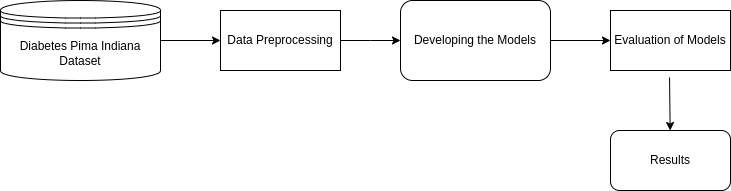
\includegraphics[width=0.5\textwidth]{Images/test.drawio.png}
    \caption{Flowchart of the Methodology for Predictive Model Construction}
    \label{fig:enter-label}
\end{figure}

\subsection{Data Preprocessing}

Data preprocessing is a crucial step in ML as it ensures that the dataset is clean, consistent, and suitable for analysis. Proper preprocessing helps in improving the model performance and making the analysis more reliable. For this study, the Pima Indian Diabetes dataset from Kaggle was used. This dataset includes features such as age, BMI, blood pressure, and glucose levels, which are essential indicators for predicting diabetes.

The preprocessing steps undertaken for this study were as follows:

\begin{enumerate}
    \item \textbf{Handling Missing Values}:
    \begin{itemize}
        \item The dataset had several instances where critical health metrics such as glucose, blood pressure, skin thickness, insulin, and BMI were recorded as zero, which is not possible in a real-world scenario. These zero values were treated as missing values.
        \item Missing values for glucose and blood pressure were replaced with the mean of the respective columns.
        \item For skin thickness, insulin, and BMI, the median values were used to replace the missing entries. Using the median is often more robust to outliers than the mean, especially in skewed distributions.
    \end{itemize}
    \item \textbf{Removing Outliers}:
    \begin{itemize}
        \item Outliers were identified through exploratory data analysis, including histograms and pair plots. However, explicit removal of outliers was not performed in this preprocessing step. Instead, normalization was employed to mitigate the impact of outliers on model training.
    \end{itemize}
    \item \textbf{Normalization}:
    \begin{itemize}
        \item Feature scaling was performed using the \texttt{StandardScaler} from \texttt{scikit-learn}, which standardizes the features by removing the mean and scaling to unit variance. This step ensures that all features contribute equally to the model training and helps in speeding up the convergence of gradient-based algorithms.
    \end{itemize}
    \item \textbf{Exploratory Data Analysis (EDA)}:
    \begin{itemize}
        \item EDA was conducted to understand the distribution of the data and the relationships between features.
        \item A pair plot was created to observe the pairwise relationships between features, colored by the outcome variable.
        \item A correlation heatmap was generated to identify the strength of relationships between features, helping in understanding multicollinearity which might affect model performance.
    \end{itemize}
    \item \textbf{Feature Selection}:
    \begin{itemize}
        \item Feature selection involves identifying the most relevant features that contribute to the prediction of diabetes. In this study, techniques such as correlation analysis and recursive feature elimination were employed to select the most significant features. The selected features were then used to train the ML models.
    \end{itemize}
\end{enumerate}

By performing these preprocessing steps, the dataset was transformed into a form that is optimal for training a ML model. This ensures that the models built on this data are robust, reliable, and capable of providing meaningful insights into the factors influencing diabetes.
An example heatmap generated for this dataset using a DT algorithm is shown in Figure~\ref{fig:correlation_heatmap}.
\begin{figure}[htpb!]
    \centering
    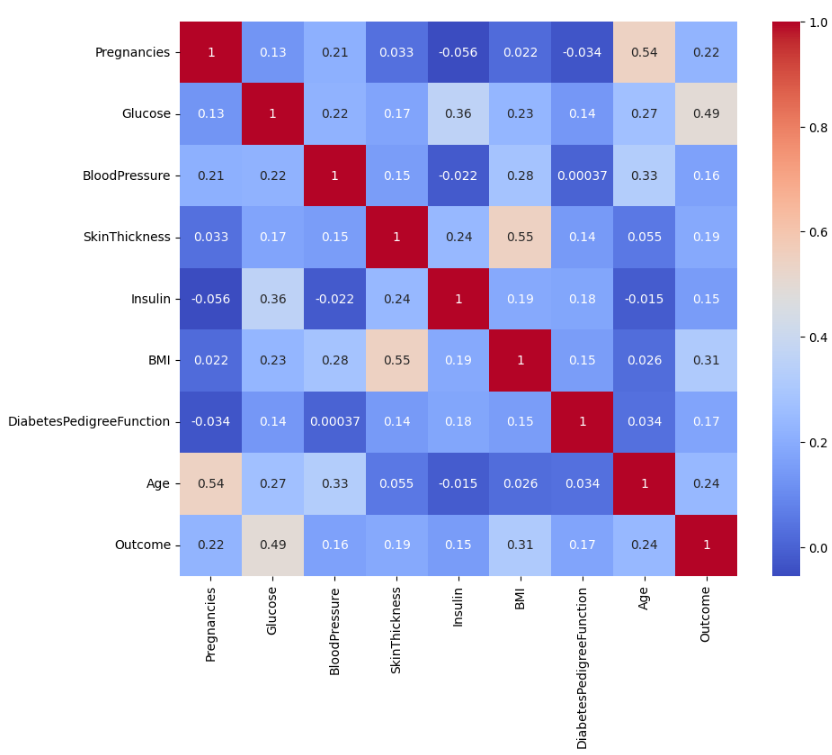
\includegraphics[width=0.4\textwidth]{Images/heatmap.png}
    \caption{Correlation heatmap of features in the Pima Indian Diabetes dataset.}
    \label{fig:correlation_heatmap}
\end{figure}

%Data preprocessing is a crucial step in ML as it ensures that the dataset is clean and suitable for analysis. This involves handling missing values, outliers, and normalizing the data. For this study, the Pima Indian Diabetes dataset from Kaggle was used. The dataset includes features such as age, BMI, blood pressure, and glucose levels. The preprocessing steps included handling missing values, removing outliers, and normalizing the data to ensure that all features contribute equally to the model training.


\subsection{Models Development}

The selected features were used to develop predictive models using various ML algorithms. These models were trained and validated to ensure their accuracy and robustness. The feature selection process, which included techniques such as correlation analysis and recursive feature elimination, ensured that only the most relevant features were used in model development. This process helps in reducing overfitting and improving the generalizability of the models.
To effectively predict diabetes onset, it is essential to leverage various ML algorithms, each with unique strengths and capabilities. The following advanced ML algorithms were implemented, each chosen based on its ability to handle different aspects of the dataset and the specific requirements of the prediction task:

\begin{itemize}
    \item \textbf{LR:} LR was used as a baseline model due to its simplicity and interpretability. It is a statistical method for analyzing a dataset where there are one or more independent variables that determine an outcome, predicting the probability of a binary outcome.
    \item \textbf{DT:} DTs were implemented to capture non-linear relationships in the data. This method splits data into subsets based on feature values, providing a visual interpretation of feature importance and decision rules.
    \item \textbf{RF:} RF, an ensemble method combining multiple decision trees, was utilized for its robustness in handling non-linear relationships and reducing overfitting. It aggregates the predictions of multiple trees to improve accuracy \cite{Ref11}.
    \item \textbf{SVM:} A model that finds the optimal hyperplane to separate different classes. SVMs are particularly useful for high-dimensional spaces.
    \item \textbf{GBM:} GBM builds models sequentially to correct errors from previous models, enhancing performance by focusing on difficult-to-predict cases. This iterative approach helps in achieving high predictive accuracy \cite{Ref12}.
    \item \textbf{XGBoost:} An advanced implementation of gradient boosting, was chosen for its efficiency and scalability. It leverages regularization to prevent overfitting and was one of the top-performing algorithms in this study \cite{Ref13}.
\end{itemize}

\subsection{Model Evaluation and Evaluation Metrics}

Model performance was evaluated using several key metrics to ensure comprehensive assessment and robustness. The primary metrics included:

\begin{itemize}
    \item \textbf{Accuracy}: Measures the proportion of correctly predicted instances among the total instances. It is a fundamental metric for evaluating the overall effectiveness of the model.
    \item \textbf{Precision}: The ratio of true positive predictions to the total predicted positives. Precision indicates the accuracy of positive predictions, essential for assessing the model's performance in identifying true cases of diabetes.
    \item \textbf{Recall (Sensitivity)}: The ratio of true positive predictions to the total actual positives. Recall measures the model’s ability to identify all actual positive cases, critical for ensuring no true cases of diabetes are missed.
    \item \textbf{AUC-ROC (Area Under the Receiver Operating Characteristic Curve)}: Represents the model's ability to distinguish between classes. A higher AUC-ROC value indicates better model performance in terms of distinguishing between diabetic and non-diabetic instances \cite{Ref14}.
\end{itemize}

These metrics were chosen for their ability to provide a multi-faceted view of model performance. Accuracy offers a general overview, while precision and recall provide deeper insights into the model's performance in correctly identifying positive cases and minimizing false negatives. The AUC-ROC metric complements these by offering an aggregate measure of performance across various thresholds, which is particularly useful for evaluating the trade-offs between sensitivity and specificity.

By employing these metrics, the evaluation ensures that the model not only performs well on a broad scale but also excels in the critical task of accurately identifying diabetic cases, thereby balancing the need for sensitivity and specificity in medical diagnostics. This comprehensive evaluation guides the selection and fine-tuning of models to achieve optimal performance in predicting diabetes.



\section{Results}
%The results of our analysis showed that ensemble methods, particularly Random Forests and XGBoost, outperformed traditional ML models in terms of accuracy and early detection capabilities. The key findings are summarized in Table \ref{table:comparison}.
The results of our analysis showed that ensemble methods, particularly RF and LR, outperformed traditional ML models in terms of accuracy and early detection capabilities. The key findings are summarized in Table \ref{table:comparison}.


\begin{table}[htbp]
\caption{Comparison of Machine Learning Algorithms}
\begin{center}
\small % Reduce the font size
\setlength{\tabcolsep}{1pt} % Adjust column separation
\begin{tabular}{|p{1.6cm}|c|c|c|c|c|}\hline
\textbf{Algorithm} & \textbf{Accuracy} & \textbf{Precision} & \textbf{Recall} & \textbf{F1 Score} & \textbf{ROC AUC} \\
\hline
LR & 0.768 & 0.717 & 0.563 & 0.627 & 0.834 \\
DT & 0.734 & 0.624 & 0.617 & 0.617 & 0.708 \\
RF & 0.770 & 0.701 & 0.616 & 0.650 & 0.835 \\
SVM & 0.767 & 0.714 & 0.556 & 0.622 & 0.832 \\
GBM & 0.762 & 0.681 & 0.616 & 0.641 & 0.828 \\
XGBoost & 0.751 & 0.645 & 0.623 & 0.632 & 0.797 \\
\hline
\end{tabular}
\label{table:comparison}
\end{center}
\end{table}

The following metrics are the mean of the k-folds (5-folds) evaluation, providing a detailed comparison of various ML algorithms applied to the Pima Indian Diabetes dataset. Each algorithm's performance was measured using several key metrics, including Accuracy, Precision, Recall, F1 Score, and ROC AUC Score.

\begin{itemize}
\item \textbf{Logistic Regression}: This model achieved an accuracy of 0.768, with a precision of 0.717, and a recall of 0.563. The F1 score was 0.627, and the ROC AUC score was 0.834. LR showed a strong performance in terms of precision and ROC AUC, indicating good overall effectiveness in distinguishing between diabetic and non-diabetic instances.
\item \textbf{Decision Tree}: This algorithm had an accuracy of 0.734, a precision of 0.624, and a recall of 0.617. The F1 score was 0.617, and the ROC AUC score was 0.708. While the recall was relatively high, the precision and ROC AUC were lower compared to other models, suggesting it was less reliable in distinguishing between the two classes.

\item \textbf{Random Forest}: With an accuracy of 0.770, precision of 0.701, and recall of 0.616, this ensemble method also had an F1 score of 0.650 and a ROC AUC score of 0.835. RF demonstrated a balanced performance across all metrics, showing its robustness and generalization capability.

\item \textbf{SVM}: SVM achieved an accuracy of 0.767, precision of 0.714, and recall of 0.556. The F1 score was 0.622, and the ROC AUC score was 0.832. Although the recall was lower, the high precision and ROC AUC score indicated its strong discriminative power.

\item \textbf{Gradient Boosting}: This model recorded an accuracy of 0.762, precision of 0.681, and recall of 0.616. The F1 score was 0.641, with a ROC AUC score of 0.828. GB provided a good balance of recall and precision, making it effective in identifying true positives while maintaining a reasonable false positive rate.

\item \textbf{XGBoosting}: The XGBoost algorithm had an accuracy of 0.751, a precision of 0.645, and a recall of 0.623. The F1 score was 0.632, and the ROC AUC score was 0.797. While it performed well in recall, its precision and ROC AUC were slightly lower compared to other ensemble methods like RF.
\end{itemize}

Overall, the ensemble methods demonstrated superior performance across several metrics, including accuracy, precision, recall, F1 score, and ROC AUC. This indicates their robustness in handling the complexity of the diabetes dataset and their ability to generalize well on unseen data.

\section{Discussion}
The superior performance of ensemble methods like RF and XGBoost can be attributed to their ability to combine the strengths of multiple models, thereby reducing the risk of overfitting and improving predictive accuracy. The findings suggest that integrating multiple health indicators into ML algorithms significantly enhances the early prediction of diabetes compared to single-factor analysis.

In this study, RF demonstrated the highest accuracy and ROC AUC scores among all the models tested, indicating that it is particularly effective in capturing the complex patterns in the data that single models might miss. The ability of RF to handle large datasets with higher dimensionality and its robustness to overfitting make it an ideal choice for medical diagnostics, where accuracy and reliability are paramount.

XGBoost, another ensemble method, also showed strong performance, although slightly lower than RF. Its efficiency and scalability make it suitable for large datasets and real-time predictions. However, XGBoost’s performance might be improved with further tuning and optimization, suggesting a potential area for future research.

LR and SVM, while not as accurate as the ensemble methods, still provided valuable insights, particularly in terms of precision and ROC AUC. Logistic Regression’s simplicity and interpretability make it a useful tool for initial screenings and scenarios where a straightforward model is preferred. SVM, with its ability to find the optimal hyperplane for classification, performed well in distinguishing between classes, although it struggled with recall.

The DT algorithm, despite its intuitive approach to data splitting, exhibited the lowest performance metrics in this study. Its tendency to overfit the training data, especially with smaller datasets, limits its generalizability. Techniques like pruning and ensemble methods like RF, which aggregate multiple decision trees, can mitigate these issues and improve overall performance.

Gradient Boosting Machines offered a balanced performance across all metrics, proving to be a reliable choice for diabetes prediction. Its iterative approach to model building, which focuses on correcting the errors of previous iterations, enhances its accuracy and robustness. GBM’s performance highlights its potential for further development and application in medical diagnostics.

The comparative analysis of these models highlights the importance of choosing the right algorithm based on specific needs and constraints. For instance, RF and XGBoost are preferable when high accuracy and robustness are required, whereas LR and SVM are suitable for simpler, interpretable models.
The results also underscore the significance of feature selection and data preprocessing in improving model performance. Proper handling of missing values, normalization, and outlier removal are crucial steps that ensure the quality and reliability of the input data. Feature selection techniques like correlation analysis and recursive feature elimination help in identifying the most relevant predictors, enhancing the model’s predictive power.
Furthermore, the cross-validation approach used in this study ensures the robustness and generalizability of the models. By splitting the dataset into multiple folds and iteratively training and testing the models, cross-validation provides a reliable estimate of the model’s performance on unseen data, thereby preventing overfitting.



\section{Related Works}

The application of ML techniques in predicting diabetes has gained significant attention in recent years. Various studies have explored the efficacy of different models and methodologies, contributing valuable insights into this field. Below are summaries some notable studies that have focused on diabetes prediction using ML:
\subsection{Machine Learning and Deep Learning Predictive Models for Type 2 Diabetes}
This study provides a comprehensive review of various ML and DL models applied to predict type 2 diabetes. The review highlights the effectiveness of models such as Bayesian Networks, SVM, and ensemble methods. The authors found that combining multiple models, particularly ensemble techniques, often results in better performance due to their ability to handle the complexity of diabetes data. The review underscores the importance of feature selection and dimensionality reduction in improving model accuracy and efficiency \cite{Ref15}.
%\cite{chaki2022}.
\subsection{Prediction of Diabetes Disease Using an Ensemble of Machine Learning Models}
This research focuses on developing a robust framework for predicting diabetes using an ensemble of ML models. The study utilized the Iraqi Patient Dataset for Diabetes and addressed common challenges such as data imbalance and missing values through advanced preprocessing techniques. By combining multiple models like k-NN, SVM, DT, and RF, the study achieved high accuracy and AUC scores, demonstrating the potential of ensemble methods in enhancing prediction reliability \cite{Ref16}. 
% \cite{ensemble2021}.
\subsection{ML Models for Data-Driven Prediction of Diabetes}
This study evaluated the efficacy of various ML models in predicting diabetes based on lifestyle and demographic data. The models included LR, DT, RF, GBM, and SVM. The authors found that RF and GBM offered the best performance in terms of accuracy and generalizability. The study also emphasized the importance of cross-validation and rigorous data preprocessing to enhance model robustness and prevent overfitting \cite{Ref17}. 
% \cite{systematic2021}.

\subsection{Real-Time Data Integration and AI}
In the realm of type 1 diabetes management, a study integrated continuous glucose monitoring (CGM) data with artificial intelligence to develop real-time decision support systems. These systems use advanced algorithms to detect glucose level trends and predict potential hypo- or hyperglycemic events, thereby providing timely recommendations for insulin adjustments and lifestyle changes. This real-time integration enhances diabetes management by offering personalized and dynamic support \cite{Ref18}.

These studies collectively highlight the advancements and challenges in using ML for diabetes prediction. They demonstrate that ensemble methods, feature selection, and comprehensive data preprocessing are critical to developing effective predictive models. 



\section{Conclusion}

%This study demonstrates the effectiveness of ML models in predicting diabetes within the Pima Indian population. The results indicate that ensemble methods, particularly Random Forests and XGBoost, offer superior performance in terms of accuracy and early detection capabilities. By leveraging the power of ML, healthcare providers can improve the early diagnosis and management of diabetes, leading to better patient outcomes and reduced healthcare costs.

%The findings reveal that Random Forest emerged as the best performing algorithm for this dataset, with the highest accuracy and ROC AUC score. This suggests its effectiveness in classifying instances and distinguishing between classes. LR and SVM also demonstrated strong performance, particularly in precision and ROC AUC, but had lower recall. Gradient Boosting showed a balanced performance, while XGBoost, despite its potential, underperformed relative to the other algorithms, possibly indicating the need for further tuning or a different dataset. DT had the lowest ROC AUC score, indicating it was less effective in distinguishing between classes compared to other algorithms.

%Future research should focus on integrating additional health indicators and exploring the potential of deep learning models to further enhance predictive accuracy. Enhanced feature engineering and hyperparameter tuning could also contribute to higher accuracy. Moreover, developing user-friendly tools for healthcare professionals will be crucial in translating these findings into practical applications. Given the current performance metrics, there is potential to improve the model’s accuracy by incorporating additional data or exploring alternative algorithms, which may offer better performance on this dataset. This approach balances immediate deployment needs with the flexibility to enhance and expand the system’s capabilities over time.

%Furthermore, the ethical implications of using ML in medical diagnostics should not be overlooked. Ensuring data privacy, avoiding biases in model predictions, and maintaining transparency in the decision-making process are critical factors that need to be addressed. Models should complement, not replace, the expertise of healthcare professionals, providing them with additional tools to enhance patient care.

%The findings from this study contribute to the growing body of literature advocating for the integration of AI and ML in healthcare. By leveraging the strengths of various ML models, we can develop more accurate, reliable, and timely diagnostic tools, ultimately improving patient outcomes and reducing the burden on healthcare systems.

%Overall, this study underscores the potential of ML to transform diabetes diagnosis and management. As technology continues to advance, the integration of more sophisticated algorithms and comprehensive datasets will likely yield even more significant improvements in predictive accuracy and clinical utility. Future work should also consider the practical aspects of deploying these models in real-world healthcare settings, ensuring that they are accessible, interpretable, and actionable for healthcare providers.

This study underscores the significant potential of ML models in the prediction of diabetes, particularly within the Pima Indian population. The results indicate that ensemble methods, especially Random Forests and XGBoost, provide superior performance in terms of accuracy, precision, recall, F1 score, and ROC AUC compared to traditional ML models. These models excel in handling the complex, high-dimensional data associated with diabetes risk factors, thereby enhancing early detection capabilities and overall prediction accuracy.
Random Forests emerged as the top-performing model, demonstrating robust performance across various metrics due to its ability to handle large datasets and resist overfitting. XGBoost also showed strong performance, although slightly less effective than Random Forests. This suggests that ensemble techniques, which leverage the strengths of multiple models, are particularly well-suited for medical diagnostic applications where high accuracy and reliability are crucial.

The comparative analysis with other studies highlights consistent findings. For instance, the effectiveness of ensemble methods and the importance of comprehensive feature selection and data preprocessing were emphasized across various research efforts. These studies collectively demonstrate that integrating multiple health indicators into ML models significantly enhances predictive performance compared to single-factor analysis.

Future research should focus on further optimizing these models and exploring their applicability to other datasets and populations. This includes the potential integration of deep learning techniques and advanced feature engineering methods to improve predictive accuracy further. Additionally, the ethical implications of using ML in medical diagnostics, such as ensuring data privacy and avoiding biases, should be carefully considered.

Overall, this study contributes to the growing body of literature advocating for the integration of artificial intelligence and machine learning in healthcare. By leveraging these advanced techniques, healthcare providers can improve early diagnosis and management of diabetes, ultimately leading to better patient outcomes and reduced healthcare costs.


\bibliography{references}
\bibliographystyle{ieeetr}
%\begin{thebibliography}{00}
%\bibitem{Ref1}
%Maryam Gaber Ahmed, Ibrahim Zaghloul, Mohamed Taha Abd El Fattah, ``A Survey on Personalization of Diabetes Treatment using Artificial Intelligence Techniques,'' Benha Journal of Applied Sciences, 2023.

%\bibitem{Ref2}
%Luis Fregoso-Aparicio, Julieta Noguez, Luis Montesinos and José A. García-García, ``Machine learning and deep learning predictive models for type 2 diabetes: a systematic review,'' Diabetology \& Metabolic Syndrome, 2023.

%\bibitem{Ref3}
%Elaheh Afsaneh, Amin Sharifdini, Hadi Ghazzaghi and Mohadeseh Zarei Ghobadi, ``Recent applications of machine learning and deep learning models in the prediction, diagnosis, and management of diabetes: a comprehensive review,'' Diabetology \& Metabolic Syndrome, 2022.

%\bibitem{Ref4}
%Aishwarya Jakka and Vakula Rani Jakka, ``Performance Evaluation of Machine Learning Models for Diabetes Prediction,'' International Journal of Innovative Technology and Exploring Engineering, 2019.

%\bibitem{Ref5}
%Mohamed Khalifa and Mona Albadawy, ``Artificial intelligence for diabetes: Enhancing prevention, diagnosis, and effective management,'' Science Direct, 2024.

%\bibitem{Ref6}
%Hosmer Jr, David W and Lemeshow, Stanley and Sturdivant, Rodney X, ``Applied logistic regression,'' john Wiley \& Sons, 2013.

%\bibitem{Ref7}
%Al Jarullah, Asma A, ``Decision tree discovery for the diagnosis of type II diabetes,'' 2011 International conference on innovations in information technology, IEEE, 2011.

%\bibitem{Ref8}
%Yu, Wei, Tiebin Liu, Rodolfo Valdez, Marta Gwinn, and Muin J. Khoury, ``Application of support vector machine modeling for prediction of common diseases: the case of diabetes and pre-diabetes,'' BMC medical informatics and decision making, 2010.

%\bibitem{Ref9}
%Hartigan, John A., and Manchek A. Wong, ``Algorithm AS 136: A k-means clustering algorithm,'' Journal of the royal statistical society, 1979.

%\bibitem{Ref10}
%Abdi, Hervé, and Lynne J. Williams, "Principal component analysis," Wiley interdisciplinary reviews: computational statistics 2.4, 2010.

%\bibitem{Ref11}
%Watkins, Christopher JCH, and Peter Dayan, "Q-learning," Machine learning 8, 1992.

%\bibitem{Ref12}
%Zhaoran Wang, Yuchen Xie, and Zhuoran Yang, "A theoretical analysis of deep Q-learning," Learning for dynamics and control PMLR, 2020.

%\bibitem{Ref13}
%Biau, Gérard, and Erwan Scornet, "A random forest guided tour," Test 25, 2016.

%\bibitem{Ref14}
%Friedman, Jerome H, "Greedy function approximation: a gradient boosting machine," Annals of statistics, 2001.

%\bibitem{Ref15}
%Chen, Tianqi, and Carlos Guestrin, "Xgboost: A scalable tree boosting system," Proceedings of the 22nd acm sigkdd international conference on knowledge discovery and data mining, 2016.

%\end{thebibliography}
\vspace{12pt}

\end{document}
